\chapter*{Introduzione}

Un punto di partenza fondamentale per lo studio della materia è la distinzione, nonché il profondo legame, tra il concetto di \textbf{Privacy} e quello di \textbf{Data Protection} (Protezione dei dati), sanciti nella Carta dei diritti fondamentali dell'Unione Europea:
\begin{itemize}
    \item \textbf{Articolo 7 - Rispetto della vita privata e della vita familiare:} Sancisce la nascita e il riconoscimento formale della privacy. La privacy viene qui definita come un vero e proprio \textbf{diritto fondamentale del cittadino}, ovvero il diritto a non subire ingerenze non giustificate nella propria sfera privata.
    \item \textbf{Articolo 8 - Protezione dei dati di carattere personale:} Introduce il concetto di \textit{Data Protection}. La protezione dei dati non è semplicemente una regola tecnica, ma è il \textbf{modo pratico per realizzare e tutelare la privacy}. Affinché il trattamento dei dati (\textit{data processing}) sia lecito, è necessario che vi sia il \textbf{consenso inequivocabile e chiaro} della persona interessata. Inoltre, questo articolo garantisce all'individuo il diritto inalienabile di poter accedere e visionare i propri dati raccolti da terzi.
\end{itemize}

Questa distinzione ci porta a chiarire un ulteriore dualismo, spesso fonte di confusione: quello tra \textit{Security} (Sicurezza) e \textit{Privacy} (Riservatezza). Sebbene siano spesso confusi, affrontano problemi diversi. Mentre la sicurezza si concentra sulle misure tecniche atte a proteggere i dati da accessi non autorizzati e attacchi informatici, la privacy riguarda il diritto dell'utente di controllare l'uso che viene fatto delle proprie informazioni. Un sistema può essere tecnicamente molto sicuro, ma violare comunque la privacy degli utenti se raccoglie e utilizza dati senza un consenso trasparente.

Proprio per restituire all'utente il controllo sulle proprie informazioni, le normative moderne conferiscono ai cittadini strumenti potenti. Tra i diritti dell'interessato spiccano in particolare:
\begin{itemize}
    \item \textbf{Diritto alla cancellazione (o Diritto all'oblio):} Consente all'utente di richiedere e ottenere l'eliminazione definitiva dei propri dati personali dai sistemi di un'organizzazione.
    \item \textbf{Diritto alla portabilità:} La possibilità per l'utente di ricevere i propri dati in un formato strutturato e di trasferirli facilmente da un fornitore di servizi a un altro (es. da un social network all'altro).
\end{itemize}

La corretta gestione di queste complesse dinamiche all'interno delle aziende richiede l'intervento di figure professionali con responsabilità ben distinte e complementari:
\begin{itemize}
    \item \textbf{CTO (Chief Technology Officer):} Ha la responsabilità dell'infrastruttura tecnologica e delle scelte di sviluppo IT dell'azienda.
    \item \textbf{CISO (Chief Information Security Officer):} È il responsabile della sicurezza informatica pura. Si assicura che le reti e i sistemi aziendali siano protetti contro intrusioni, malware e data breach.
    \item \textbf{DPO (Data Protection Officer):} È il responsabile della protezione dei dati. Rispetto al CISO, il DPO affronta \textbf{problematiche molto più ampie e trasversali}. Non si limita a verificare la solidità dei firewall, ma deve garantire che l'intera organizzazione rispetti le normative (come il GDPR). È la figura che si occupa attivamente di gestire i diritti degli utenti, come ad esempio supervisionare le pratiche legali e tecniche per garantire l'\textbf{eliminazione} dei dati o consentirne il corretto \textbf{accesso} all'utente che ne fa richiesta.
\end{itemize}

\chapter{Symmetric Needham-Schroeder e Kerberos}
Passiamo ora ad analizzare il protocollo \textbf{Symmetric Needham-Schroeder}, che pone le basi teoriche e strutturali per quello che sarà poi Kerberos. Ci troviamo in un contesto di crittografia simmetrica, in cui ogni entità condivide una chiave segreta a "lungo termine" con un Trusted Third Party (TTP). Lo scopo del protocollo è permettere al TTP di generare e distribuire in modo sicuro una chiave di sessione ($K_{ab}$) affinché due nodi, $A$ e $B$, possano comunicare.

Il protocollo si sviluppa nei seguenti cinque passaggi:
\begin{align*}
    1.\quad & A \rightarrow TTP : A, B, N_a \\
    2.\quad & TTP \rightarrow A : \{N_a, B, K_{ab}, \{K_{ab}, A\}_{K_b}\}_{K_a} \\
    3.\quad & A \rightarrow B : \{K_{ab}, A\}_{K_b} \\
    4.\quad & B \rightarrow A : \{N_b\}_{K_{ab}} \\
    5.\quad & A \rightarrow B : \{N_b - 1\}_{K_{ab}}
\end{align*}

Analizzando la struttura di questo scambio di messaggi, emergono alcuni dettagli e criticità importanti:
\begin{itemize}
    \item \textbf{Freshness e prevenzione dei Replay Attack:} I passaggi 4 e 5 servono a $B$ per ottenere garanzia di \textit{freshness} sulla chiave di sessione appena ricevuta. L'operazione di decurtazione (il $-1$ applicato alla nonce $N_b$ nel passaggio 5) è fondamentale per differenziare i due messaggi; se fossero identici, un attaccante potrebbe semplicemente intercettare il messaggio 4 e rispedirlo identico al mittente.
    \item \textbf{Mancanza di Explicitness:} Il protocollo pecca nel principio di esplicitezza. Al passaggio 4, $A$ riceve un messaggio crittografato ma non ha la prova esplicita di chi glielo stia mandando. Similmente, quando $B$ riceve la nonce indietro al passaggio 5, \textit{presume} che sia stata elaborata e inviata da $A$, ma il messaggio in sé non ne contiene l'identità.
\end{itemize}

Queste vulnerabilità aprono le porte a un attacco critico se consideriamo un modello di minaccia più avanzato. Introduciamo quindi l'attaccante \textbf{Dolev-Yao Plus}, un'estensione del classico modello Dolev-Yao in cui l'attaccante non solo può intercettare, bloccare e falsificare i messaggi, ma è anche riuscito a impossessarsi di vecchie chiavi di sessione ormai compromesse.

Sfruttando una vecchia chiave di sessione ($K_{ab}$) e il relativo ticket crittografato ($\{K_{ab}, A\}_{K_b}$), l'attaccante $C$ può perpetrare un \textbf{Replay Attack} (noto anche come attacco di Denning-Sacco) riutilizzando il passaggio 3 e impersonando $A$:
\begin{align*}
    3.\quad & C \rightarrow B : \{K_{ab}, A\}_{K_b} && \text{(Ticket vecchio intercettato precedentemente)} \\
    4.\quad & B \rightarrow C : \{N_b'\}_{K_{ab}} && \text{(B risponde all'attaccante credendo sia A)} \\
    5.\quad & C \rightarrow B : \{N_b' - 1\}_{K_{ab}} && \text{(C, conoscendo la vecchia chiave, calcola la risposta)}
\end{align*}

Il cuore del problema risiede nel messaggio 5. Questo messaggio dimostra a $B$ soltanto che "qualcuno che conosce la chiave di sessione ha letto e processato la nonce". Non si tratta di un problema di autenticazione in senso stretto (che si risolverebbe aggiungendo i nomi all'interno dei messaggi crittografati per garantire l'esplicitezza), bensì di un problema di \textbf{freshness dell'autenticazione}: $B$ non ha alcuna garanzia che la richiesta di sessione sia \textit{attualmente} voluta da $A$.

Per mitigare questa falla strutturale, la soluzione consiste nell'includere una nonce generata da $B$ fin dall'inizio nella produzione della chiave di sessione.
\begin{align*}
    1.\quad & A \rightarrow B : A \\
    2.\quad & B \rightarrow A : \{A, N'_b\}_{K_{b}} \\
    3.\quad & A \rightarrow TTP : A, B, N_a, \{A, N'_b\}_{K_b} \\
    4.\quad & S \rightarrow A: \{N_a,K_{ab}, B,\{K_{ab}, A, N'_b\}_{K_b} \}
\end{align*}
Per risolvere il problema della freschezza dell'autenticazione emerso con il protocollo Needham-Schroeder, si è resa necessaria un'evoluzione. Vogliamo un protocollo sicuro che risolva i limiti del precedente: per farlo, si passò dall'uso delle nonce all'utilizzo dei \textbf{timestamp}. Sebbene all'epoca l'uso dei timestamp non fosse considerato pratico principalmente per le difficoltà legate alla sincronizzazione degli orologi tra macchine diverse, il protocollo \textbf{Denning-Sacco} fu il primo a implementarli con successo. Questo filone di ricerca gettò le basi per il \textbf{Progetto Athena} del MIT, dal quale è nato il protocollo che oggi conosciamo come \textbf{Kerberos}.


Progettare un sistema di sicurezza per una rete locale (LAN) impone di trovare il giusto compromesso tra \textbf{Autenticazione} e \textbf{Usabilità}. L'obiettivo è permettere agli utenti di accedere in maniera sicura ai vari servizi offerti dalla nostra LAN. 

Tuttavia, emerge subito un problema di usabilità: se ogni accesso a un nuovo servizio di rete causasse una nuova procedura di autenticazione, l'esperienza utente sarebbe inefficiente poiché dovrebbe reinserire di volta in volta le sue credenziali. La soluzione a questo problema è l'adozione di un meccanismo di \textbf{Single Sign-On (SSO)}.
Analizziamo i concetti chiave del Single Sign-On:
\begin{itemize}
    \item \textbf{Definizione:} Il Single Sign-On consiste nell'usare un'unica credenziale di autenticazione per accedere a tutti i servizi. In pratica, l'utente si autentica una sola volta all'inizio della sessione ricevendo un "token" o "ticket" che gli garantirà automaticamente l'accesso trasparente a tutti i servizi distribuiti successivi.
    \item \textbf{Il problema della robustezza:} Di base, l'SSO è una soluzione indubbiamente comoda, ma intrinsecamente poco robusta se implementata in modo ingenuo, poiché si riduce ad avere un'unica password per tutto. Se un attaccante compromettesse quell'unica credenziale, avrebbe accesso all'intero ecosistema.
\end{itemize}

Kerberos è un protocollo reale che si occupa di risolvere questo esatto problema implementando il Single Sign-On proteggendo le credenziali attraverso l'uso di ticket crittografati a tempo che fanno uso di \textbf{timestamp}. 

\section{Kerberos}
Prima di parlare di Kerberos, mostriamo una prima versione detta \textbf{BAN Kerberos} che ha uno schema molto simile a quello che vedremo successivamente.
\begin{align}
    &A \rightarrow TTP : A\\
    &TTP \rightarrow A : \{K_{ab}, B, T_k, \{K_{ab},A, T_k\}_{K_b}\}_{K_a}\\
    &A \rightarrow B : \{K_{ab}, A, T_k\}_{K_b}
\end{align}

Come già detto, Kerberos si pone come obiettivo quello di realizzare un sistema a Single Sign-On che permette una \textbf{singola autenticazione} al sistema ma che faccia un \textbf{controllo delle autorizzazioni} quando l'utente vuole accedere a specifici punti del sistema.  

Questo, inoltre, fa uso di timestamp che si differenziano dalle Nonce principalmente per il fatto che la nonce dà garanzia a chi la mette della frehness di colui che la rimanda indietro poiché prima di quel momento la nonce non era stata creata. Il timestamp, invece, non dà alcuna garanzia a colui che la riceve che questa sia veritiera poiché colui che la manda potrebbe essere malevolo e mandare un timestamp più nuovo. Se, da una parte, abbiamo delle Nonce che ci indicano chiavi "vecchie" che sono insicure, dall'altra abbiamo i Timestamp che indicano chiavi "scadute" che sono insicure. La differenza sta nel fatto che una chiave "vecchia" non ci sta a indicare un qualche riferimento temporale in termini di tempo mentre, invece, quando la scadenza dettata dal timestamp ci fissa un limite preciso nel tempo. 
Dunque, adesso che utilizzeremo i timestamp, ci fideremo solo di quelli generati da un entità fidata. 
Gli obiettivi di Kerberos sono segretezza, autenticazione ad accesso singolo e temporalità che ci permette di prevenire replay. La struttura base di Kerberos è la seguente:
\begin{figure}[H]
    \centering
    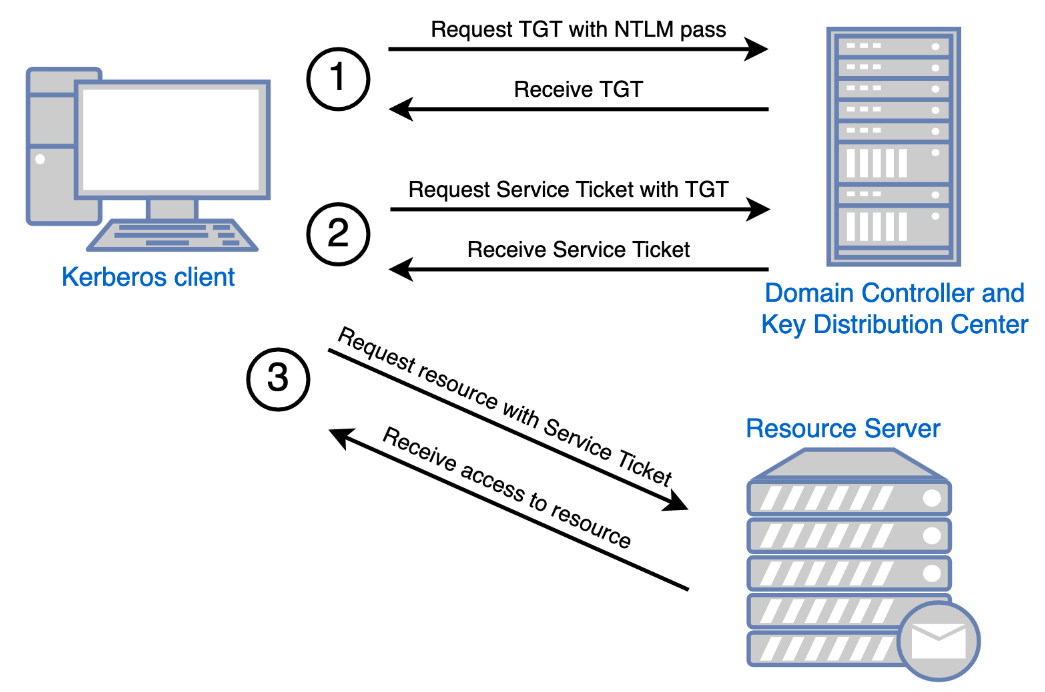
\includegraphics[width=0.5\linewidth]{Images/capitolo_1/kerberos_struttura.png}
\end{figure}
Come possiamo notare, abbiamo principalmente tre fasi:
\begin{enumerate}
    \item \textbf{Autenticazione}: Il client si autentica con l'authentication server (AS). Questa fase fornirà al client l'\textbf{AuthKey} che sarebbe la chiave di sessione per comunicare con il TGS e l'\textbf{AuthTicket} che sarebbe un ticket che A invierà al TGS per comunicargli la chiave di sessione. Questo Ticket sarà cifrato con la chiave privata del TGS così ché il client che la richiede non possa modificarlo.
    \item \textbf{Autorizzazione:} Il client chiede al Ticket Granting Server (TGS) un ticket per uno specifico servizio. Nello stesso identico modo di prima, il TGS fornisce al client la \textbf{ServKey} e il \textbf{ServTicket}.
\end{enumerate}
L'unica operazione obbligatoria è la prima mentre l'operazioni due e tre vengono effettuate solo se richieste dal client poiché non è detto che questo richieda dei servizi. 
Inoltre, con l'aggiunta dei Timestamp diventa anche necessario parlare di tempo di validità delle sessioni e delle chiavi. Infatti, con l'aggiunta dei timestamp nasce il concetto di "accetto questa operazione solo se il timestamp ha un valore minore rispetto a quello che sono disposto ad accettare". Dunque, per realizzare il Single Sign-On, avremo le credenziali di autenticazione hanno una valenza di circa 8 ore che sarebbero le ore di una tipica giornata lavorativa mentre, invece, le credenziali per i servizi hanno una valenza di al massimo qualche minuto poiché abbiamo la necessità che queste siano fresche per prevenire grosse compromissioni del sistema. 
Lo schema Kerberos funziona come segue:
\begin{align*}
    \textbf{Autenticazione:}\\
    &1. A \rightarrow AS: A, TGS, T_1\\
    &2. AS \rightarrow A: \{authK, TGS, T_a, \{A,TGS, authK,T_a\}_{K_{tgs}}\}_{K_a}\\
    \textbf{Autorizzazione:}\\
    &3. A \rightarrow TGS: \{A,TGS,authK, T_a\}_{K_{tgs}}, \{A, T_2\}_{authK}, B\\
    &4. TGS \rightarrow A: \{servK, B, T_s,\{A,B,servK,T_s\}_{K_b}\}_{authK}\\
    \textbf{Servizio:}\\
    &5. A \rightarrow B: \{A,B, servK,T_s\}_{K_b}, \{A,T_3\}_servK\\
    &6 B \rightarrow A: \{T_3 + 1\}_{servK}
\end{align*}
L'AuthTicket e il ServTicket che dicevamo prima sono rispettivamente $\{A,TGS, authK,T_a\}_{K_{tgs}}$ e $\{A,B, servK,T_s\}_{K_b}$. 
Da qui possiamo fare alcune considerazioni:
\begin{itemize}
    \item \textbf{Perché T1,T2 e T3}: se, come abbiamo detto, ci fidiamo solo di timestamp creati da entità fidate, a quale scopo inserire i timestamp nei messaggi di A? Infatti, possiamo notare che queste non sono effettivamente fidate, infatti abbiamo sempre timestamp inviati o dall'AS o dal TGS. Nel caso di $T_1$, questo serve ad A solo per marcare la sua richiesta e non è nemmeno cifrato, dunque è quasi una formalità. Nel caso di $T_2,T_3$ non ci si fida realmente dei timestamp, ci si fida del fatto che quelli inviati da A sono legati dalla cifratura che è, a sua volta, legata al timestamp inviato dall'entità fidata.   
    \item \textbf{Concatenazione del ticket e dell'autenticatore in 3 e 5:} Notiamo che i due messaggi sono concatenati e, sappiamo da internet security, non è possibile autenticare la concatenazione di due messaggi separati. Tuttavia, anche se un attaccante provasse a riciclare la seconda parte del messaggio, i timestamp fungerebbero da segnale d'allarme e chiunque se ne accorgerebbe. 
    \item \textbf{Perché B al messaggio 3 non è cifrato:} Il motivo per il quale "B" al messaggio 3 è inviato senza l'uso di alcun tipo di cifratura è dettato dal fatto che in realtà questa informazione non è necessario nasconderla dato che anche se l'attaccante lo sostituisse, al messaggio 4 arriverebbe ad A il messaggio con la servK associata ad un altro servizio. Inoltre, anche nascondendo questa informazione, poi al messaggio 5 si scoprirebbe a quale servizio sta facendo accesso. 
    \item \textbf{Il messaggio 6: } Come nel caso di Needham Schroeder simmetrico, anche in questo caso viene utilizzato quel $+1$ per differenziare il messaggio 6 dalla seconda parte del messaggio 5 ed evitare problemi. Proprio per lo stesso motivo, quando A legge $T_3 + 1$ cifrato con la servK, questo \textbf{dedurrà} di star comunicando con B e questa deduzione può essere sfruttata da Dolev-Yao +. 
    \item \textbf{Gerarchia delle chiavi: }Come possiamo notare, al passo 4 abbiamo che cifriamo $servK$ con $authK$ di fatto legando indissolubilmente due chiavi di sessione. Infatti, nel caso in cui un attaccante riuscisse a "rubare" $authK$, questo avrebbe accesso automaticamente anche a $servK$.
    \item \textbf{Scadenza delle chiavi di sessione: }Una volta scaduta la sessione di autenticazione, che cosa accade alle chiavi di sessione dei servizi ancora attive? È naturale pensare queste semplicemente smettano di essere valide, tuttavia non è un dettaglio da trascurare poiché, nel caso in cui DY+ riuscisse a impadronirsi di $authK$ scaduta, avrebbe modo di scoprire una $servKey$ ancora valida. Dunque, è necessario prendere delle precauzioni in questo senso imponendo che la validità della servK sia limitata dalla validità di authK. \\
    Quando B si trova davanti quella servK, poiché sa che vale che $Ts + Ls \leq Ta + La$\footnote{Ts è il tempo in cui è stata generata la servK mentre Ls è il suo lifetime. Allo stesso modo vale per Ta ed La.}, sa che non può essere scaduta.
    \item \textbf{Cifratura annidata: }Una cosa che possiamo notare al passo 2 e al passo 4 è la doppia cifratura del messaggio esterno e del ticket interno. Questa trovata fa' sì che colui che poi riceve il ticket, riesca ad avere garanzia che il suo interlocutore lo abbia ricevuto pure.\footnote{Attacco che si può vedere nel protocollo Otway-Rees} Se non ci fosse questa cifratura annidata ma ci fossero solamente due messaggi e nel messaggio 3 e 5 non ci fosse l'autenticatore, un attaccante potrebbe intercettare il messaggio e inviare il Ticket al TGS/Servizio senza che A lo abbia mai ricevuto. Tuttavia, poiché è presente l'autenticatore, questo annidamento è irrilevante poiché, anche se fossero separati, l'attaccante non potrebbe riuscire a formare un messaggio 3 e 5 ben fatto poiché non avrebbe l'authKey/servKey e, quindi, colui che lo riceve capisce subito che qualcosa non è andato correttamente. Questo annidamento è stato successivamente rimosso con Kerberos V.
\end{itemize}
\subsection{L'Integrazione di Kerberos con le Smart Card}

Come già affrontato in altri ambiti (ad esempio nel corso di Internet Security), l'uso delle classiche password solleva numerose criticità: richiedono lunghezze minime, set di caratteri complessi e, soprattutto, pongono il problema fondamentale di come e dove memorizzarle in modo sicuro. 

Sebbene si possa pensare di utilizzare una password per derivare la nostra chiave a lungo termine ($K_a$), nella pratica questa non rappresenta un segreto crittograficamente forte. Anche ricorrendo a tecniche di mitigazione come l'aggiunta di un \textit{salt}, derivare una chiave realmente robusta da una stringa pensata da un essere umano rimane difficile. Ma il problema principale, lato client, è un altro: \textbf{dove possiamo memorizzare la chiave $K_a$ in maniera inattaccabile?}

La soluzione a questo problema di archiviazione è l'introduzione della \textbf{Smart Card}. Non si tratta di un semplice supporto di memoria passivo, ma di un vero e proprio "mini computer" integrato in un chip. L'utilizzo di questa tecnologia si basa su due principi fondamentali:
\begin{itemize}
    \item \textbf{Inaccessibilità della chiave:} La chiave a lungo termine $K_a$ viene iniettata e salvata all'interno del chip e \textbf{non deve mai uscire} da esso. Se la chiave venisse trasferita nella RAM del computer host per essere utilizzata, saremmo punto e a capo con i rischi di compromissione.
    \item \textbf{Elaborazione interna:} Poiché il segreto non può uscire dal chip, è la Smart Card stessa a doversi occupare di eseguire fisicamente le operazioni di cifratura e decifratura richieste dal protocollo Kerberos, restituendo al computer solo il risultato dell'operazione.
\end{itemize}
\begin{figure}[H]
    \centering
    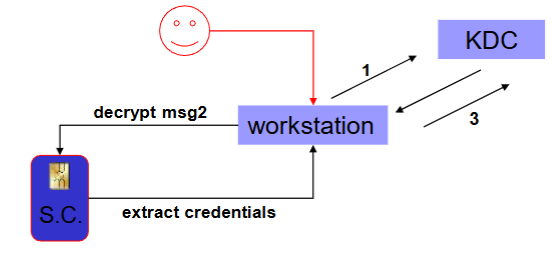
\includegraphics[width=0.75\linewidth]{Images/capitolo_1/kerberos_smartcard.png}
\end{figure}
Come possiamo osservare dal diagramma, i ruoli sono nettamente separati per garantire la sicurezza:
\begin{enumerate}
    \item Sarà la \textbf{workstation} (il computer fisico) a generare e inviare il primo messaggio in chiaro (msg 1) verso il KDC (Key Distribution Center), dichiarando la propria identità.
    \item Il KDC risponde con un messaggio crittografato (msg 2) che contiene, tra le altre cose, la chiave di sessione.
    \item A questo punto, la workstation inoltra il messaggio crittografato alla \textbf{Smart Card}.
    \item È la Smart Card (e solo lei) a possedere la chiave a lungo termine necessaria per decifrare il messaggio (\textit{decrypt msg2}).
    \item Una volta decifrato internamente il pacchetto, la Smart Card estrae le credenziali utili (\textit{extract credentials})—ovvero la nuova chiave di sessione appena generata—e le fornisce alla workstation. 
\end{enumerate}

In questo modo, la workstation ottiene la chiave di sessione temporanea necessaria per proseguire le comunicazioni, ma la chiave a lungo termine dell'utente è rimasta al sicuro, inviolata all'interno del chip della Smart Card.

È importante sottolineare l'enorme salto generazionale e di sicurezza rispetto alla precedente tecnologia delle \textbf{carte magnetiche}. Queste ultime erano intrinsecamente insicure, paragonabili a un "libro aperto": non offrivano alcuna garanzia di riservatezza e chiunque fosse dotato di un semplice lettore poteva leggerne o clonarne il contenuto senza alcuno sforzo. 

Le Smart Card (come ad esempio le \textit{Java Card}), al contrario, essendo dei dispositivi programmabili, espongono verso l'esterno solo un'interfaccia logica rigorosa. Se il software al loro interno è progettato in maniera sicura, questa interfaccia non includerà mai un comando per estrarre la chiave privata. Di conseguenza, l'unica opzione rimasta a un ipotetico attaccante per forzare una Smart Card si riduce a un complesso, costoso e distruttivo \textbf{attacco fisico} all'hardware del chip stesso.